
\chapter{Trabalhos relacionados} \label{chap:estarte}

Neste capítulo é apresentado o estudo preliminar realizado, tendo em vista a aquisição de competências e conhecimentos necessários para o desenvolvimento do projeto, que se focam essencialmente em análise de métodos de \textit{data mining} e em técnicas aplicadas em visão por computador. Em primeiro ligar será exposto conteúdo relativamente a métodos de \textit{clustering} como uma tarefa de \textit{data mining}. Em seguida será apresentado formas de representação de imagens. Por fim, são referenciados alguns trabalhos relacionados com o projeto a desenvolver nesta dissertação.

\section{Clustering} \label{sec:cluster}

Extração de conhecimento em base de dados ou \textit{Data Mining} é um processo de exploração de grande quantidades de dados que procura encontrar padrões interessantes~\citet{Han2006}. Trata-te assim de uma fusão de estatística aplicada, sistemas de lógica, inteligência artificial, \textit{Machine Learning} e gestão de base de dados~\citet{North2012}. Este processo é caracterizado por várias tarefas possíveis de ser aplicadas, dependendo do problema abordado, tais como~\citep{Fayyad1996}:

\begin{itemize}
\item Deteção de anomalias (outliers/ alterações/ desvios) - Identificação de registos de dados incomuns, podendo ser erros nos dados ou objetos interessantes que apresentam comportamento diferente dos restantes;
\item Regras de associação - Procura relações entre variáveis que ocorram frequentemente;
\item Classificação - É a tarefa de generalizar uma estrutura conhecida e aplicar a novos dados, sendo essencialmente utilizada em tarefas de previsão;
\item Regressão - Tenta encontrar uma função que se modela os dados com o mínimo de erro;
\item Resumo - Trata-se da representação mais compacta do conjunto de dados, que pode incluir visualização e descrição através de um relatório,
\item \textit{Clustering} - Tarefa de descobrir grupos em que os dados apresentam de alguma forma semelhanças, sem o uso de estruturas previamente conhecidas
\end{itemize}

Este projeto terá como principal tarefa a realização de \textit{clustering}. Pode-se definir \textit{clustering} como "um processo de agrupamento de um conjunto de objetos de dados em vários grupos ou \textit{clusters}, de modo que os objetos dentro de um \textit{cluster} apresentem alta similaridade, mas que sejam muito diferentes de objetos de outros \textit{clusters}. Diferenças e semelhanças são avaliados com base nos valores de atributos que descrevem os objetos e muitas vezes envolvem medidas de distância"~\citet{Han2006}.

A realização de \textit{clustering} é assim uma escolha lógica para a extração de padrões em dados não supervisionados e para o agrupamento de \textit{tweets} pela sua semelhança em conteúdo, neste caso as imagens, e com a integração de outras dimensões, como o tempo e espaço.

O \textit{clustering} faz parte de um conjunto de técnicas aplicadas na aprendizagem não supervisionada. Enquanto que na aprendizagem supervisionada, existe um conjunto de dados previamente analisados e rotulados que são usados para treinar um modelo para que seja capaz de encontrar relação entre os atributos desse dados com novos conjuntos dados, na aprendizagem não supervisionada, não são utilizados conjuntos de dados previamente analisados e rotulados. Assim o processo de descoberta de padrões nos dados apenas tem em conta os dados presentes, tentando organizar as instâncias em grupos semelhantes~\citet{Liu2011}.

Nesta secção serão apresentadas as principais características e técnicas para aplicação da tarefa de \textit{clustering}, tais como, \textit{clustering} por partição, \textit{clustering} hierárquico, \textit{clustering} baseado em densidade, \textit{clustering} baseado em grelhas, funções de distância para o cálculo da similaridade entre objetos e por fim, a avaliação de \textit{clusters}.


\subsection{Clustering por partição} \label{subsec:parti}

A utilização de métodos baseados em partições é a forma mais simples e elementar de realizar análise por \textit{clustering}, em que um conjunto de objetos é distribuído em vários grupos ou \textit{clusters} mais pequenos. É assumido que o número de \textit{clusters} é conhecido antes da realização da tarefa, sendo esse valor tomado como o ponto de partida para aplicação de métodos baseados em partição~\citet{Han2006}. 

\subsubsection{Algoritmo K-Means}
O algoritmo \textit{k-means} é o melhor algoritmo de \textit{clustering} por partição e o mais utilizado devido à sua simplicidade e eficiência~\citet{Liu2011}. É apresentado como  sendo  um algoritmo de \textit{clustering} por partição, pois este divide o conjunto de dados em partições mais pequenas, formando assim os \textit{clusters}.

Inicialmente é necessário que o utilizador indique o valor de \textit{k} e o algoritmo irá iterativamente dividir o conjunto de objetos em \textit{k-clusters} diferentes, baseado em funções de distância~\citet{Liu2011} que são apresentadas na subsecção~\ref{subsec:dist}.

Cada \textit{cluster} apresenta um centroide que é o representante do grupo, sendo o valor médio de todos os objetos (instâncias) pertencentes ao \textit{cluster}. Este centroide é recalculado de forma iterativa até que seja atingido o critério de paragem. A convergência ou critério de paragem pode ser um dos seguintes enumerados:

\begin{enumerate}
\item Não ocorre (ou ocorre um valor mínimo) de alterações dos objetos para diferentes \textit{clusters}.
\item Não ocorre (ou ocorre um valor mínimo) de alterações dos centroides.
\item Diminuição mínima da \textbf{soma do erro quadrático} (SEQ),
\end{enumerate}

\begin{equation}
SEQ = \sum_{j=1}^{k} \sum_{x \in C_{j} } dist(x, m_{j})^{2} ,
\end{equation}

onde \textit{k} é o número de \textit{clusters} pretendidos, $ C_{j} $ é i-íssimo \textit{cluster}, $ m_{j} $ é o centroide do \textit{cluster} $ C_{j} $ e $ dist(x, m_{j}) $ é a distância entre uma instância \textbf{x} e o centroide $ m_{j} $.

Assim, "o algoritmo \textit{k-means} pode ser usado em qualquer aplicação com um conjunto de dados onde a média pode ser definida e calculada"~\citet{Liu2011}.

No \textbf{espaço euclidiano}, o valor médio (centroide) de um \textit{cluster} é calculada da seguinte forma:

\begin{equation}
m_{j} =  \frac{1}{|C_{j}|} \sum_{x_{i} \in C_{j} }x_{i} ,
\end{equation}

onde $ |C_{j}| $ é o número de pontos (instâncias) no \textit{cluster} $ C_{j} $. A distância entre um ponto $ x_{i} $ a um centroide $ m_{j} $ é calculado da seguinte forma:

\begin{equation}
dist(x_{i}, m_{j}) = ||x_{i} - m_{j}|| =  \sqrt{(x_{i1} - m_{j1})^2 + (x_{i2} - m_{j2})^2 + ... + (x_{ir} - m_{jr})^2} .
\end{equation}

O pseudo-código deste algoritmo é apresentado no algoritmo~\ref{kmeans}.
% ESCREVER ALGORITMO

\begin{algorithm}
\caption{K-Means}\label{kmeans}
\begin{algorithmic}[1]
\Procedure{K-MEANS}{k: clusters, D: conjunto de dados}
	\State {escolher k objetos de D como centroides dos clusters iniciais;} 
	\Repeat 
		\State {(re) atribuir cada objeto a ao cluster ao qual o objeto é o mais similar;} 
		\State {actualizar o centroide do cluster;} 
	\Until{clusters sem alterações;}
	\State \textbf{return} {conjunto de k clusters;}
\EndProcedure 
\end{algorithmic}
\end{algorithm}

%\subsection{Representação de Clusters}

\subsection{Clustering hierárquico} \label{subsec:hierar}

O \textit{clustering} hierárquico é outra abordagem importante na tarefa de \textit{clustering}. Os \textit{clusters} são criados sobre a forma de uma sequência em árvore (dendrograma). Os objetos (instâncias) encontram-se no fundo do diagrama, enquanto que o conjunto de todos os objetos encontra-se no topo do diagrama. Cada nó que se encontra no interior do diagrama possui nós filhos, sendo que cada nó representa um \textit{cluster}. Assim designa-se por \textit{clusters} irmãos, aqueles que derivam de um mesmo \textit{cluster}, isto é, do nó parente~\citet{Liu2011}. A figura~\ref{fig:hierarquico} exemplifica a representação de um dendrograma. 

\begin{figure}[h]
\centering
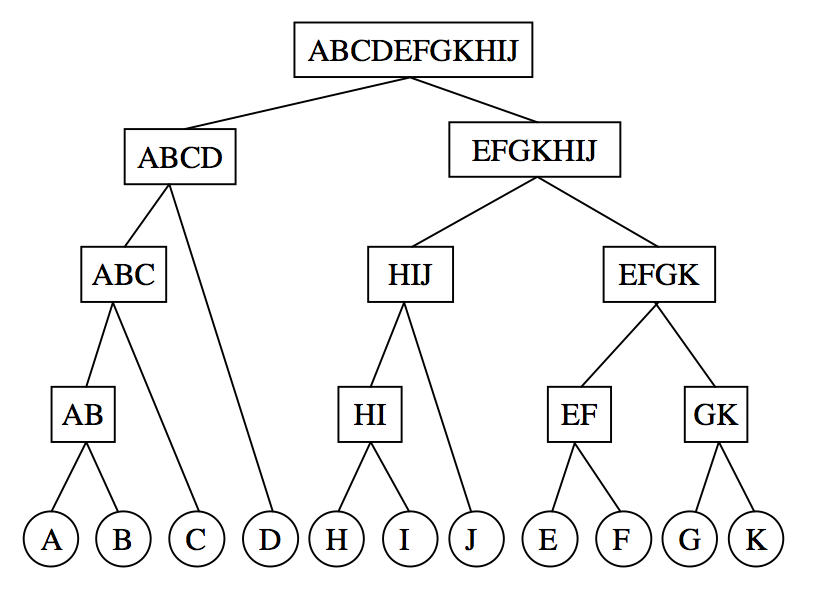
\includegraphics[width=0.6\linewidth]{./figures/hierarquico}
\caption{Dendrograma~\citet{Bramer2007}}
\label{fig:hierarquico}
\end{figure}

Existem dois tipos principais de métodos de \textit{clustering} hierárquico, sendo eles~\citet{Liu2011} :

\begin{description}
\item[\textit{Clustering} por aglomeração:] O dendrograma é construido do nível mais baixo até ao mais alto, juntando sucessivamente e iterativamente os \textit{clusters} com maiores semelhanças até existir um único \textit{cluster} com todo o conjunto dos dados.

\item[\textit{Clustering} por divisão:] O dendograma é construido do nível mais alto até ao nível mais baixo, onde o processo tem inicio com um único \textit{cluster} que possui todos os objetos, sendo dividido sucessivamente em \textit{clusters} mais pequenos, até que estes sejam constituídos apenas por um único objeto.
\end{description}

Ao contrário do algoritmo \textit{k-means}, que apenas calcula a distância entre os centroides de cada grupo ou \textit{cluster}, no \textit{clustering} hierárquico pode ser usado os vários métodos  apresentados em seguida para determinar a distância entre dois \textit{clusters}~\citet{Liu2011}: 

\begin{description}
\item[Método \textit{Single-Link}:] Neste método, a distância entre dois \textit{clusters} é determinada pela distância entre os dois objetos mais próximos (vizinhos mais próximo) pertencentes a \textit{clusters} diferentes.
\item[Método \textit{Complete-Link}:] Neste método, a distância entre dois \textit{clusters} é determinada pela maior distância entre dois objetos (vizinhos mais distante).
\item[Método Average-Link:] Este método tenta manter um compromisso entre a sensibilidade a \textit{outliers} do método \textit{Complete-Link} e a sensibilidade do método \textit{Single-Link} ao ruído existente nos dados. Para isso, é determinada a distância entre dois \textit{clusters} através da distância média entre todos os pares de objetos nos dois \textit{clusters}.
\item[Método Ward:] Este método, tenta minimizar a variância entre dois \textit{clusters} unidos.
\end{description}

Assim conclui-se que o \textit{clustering} hierárquico apresenta-se para determinados domínios, como bastante intuitivo para humanos, mas a interpretação dos resultados pode ser por vezes subjetiva. Outra característica interessante é o facto de, ao contrário do \textit{clustering} por partição, no \textit{clustering} hierárquico não ser necessário especificar logo à partida o numero de \textit{clusters}. 

\subsection{Clustering baseado em densidade} 

Os métodos de ~\textit{clustering} por partição ou hierárquico estão preparados para encontrar \textit{clusters} que apresentam formas geométricas circulares, sendo ineficiente quando as formas destes grupos são por exemplo elípticas. Assim, para descobrir \textit{clusters} com formas arbitrárias, pode ser usado métodos baseados na densidade dos objetos~\cite{Han2006}. Um dos algoritmos mais conhecidos que utiliza este tipo de método é o DBSCAN (\textit{Density-Based Spatial Clustering of Applications with Noise}) que é capaz de encontrar \textit{clusters} através da análise da densidade e proximidade dos objetos pertencentes a um conjunto de dados. Para esta análise é necessário previamente atribuir um valor que definirá o raio da vizinhança considerada para cada objeto. Esse parâmetro é designado por $ \epsilon $ e terá de ser necessariamente maior que 0. Assim,  a $ \epsilon $-vizinhança de um objeto \textit{x} é o espaço dentro de um raio com valor $ \epsilon $, centrado em \textit{x}~\cite{Han2006}. Já para determinar a densidade de uma vizinhança, é utilizado o parâmetro \textit{MinPts} também previamente definido, que especifica o número mínimo de objetos vizinhos que um objeto necessita ter em ser redor, para ser considerado como objeto central.
Os passos necessários para a implementação deste método são apresentados no algoritmo~\ref{dbscan}

\begin{algorithm}[ht]
\caption{DBSCAN}\label{dbscan}
\begin{algorithmic}[1]
\Procedure{DBSCAN}{\textit{MinPts}: limiar da vizinhança,  D: conjunto de dados, $ \varepsilon $ : raio  }
	\State {Marcar todos os objetos como não selecionados;} 
	\Repeat
		\State {escolher aleatóriamente um objeto \textit{p} não selecionado;} 
		\State {actualizar objeto \textit{p} como selecionado;} 
		\If {o $ \varepsilon$-vizinhança de \textit{p} tem pelo menos \textit{MinPts} objetos}
			\State {criar um novo \textit{cluster C} e adicionar objeto \textit{p} ao \textit{cluster C};}
			\State {Seja N o conjunto de objetos na $\varepsilon$-vizinhança de \textit{p}; }
			\For {cada ponto \textit{p'} em N}
				\If {\textit{p'} não selecionado}
					\State {Marcar \textit{p'} como selecionado}
					\If {a $\varepsilon$-vizinhança de \textit{p'} tem pelo menos \textit{MinPts}}
						\State {adicionar ponto a N}
					\EndIf
				\EndIf
				\If {\textit{p'} não pertence a nenhum cluster}
					\State {adicionar \textit{p'} a \textit{C}}
				\EndIf
			\EndFor
			\State {\textbf{output} C;}
		\Else { marcar \textit{p} como ruido}
		\EndIf
	\Until{todos os objetos selecionados;} 
\EndProcedure 
\end{algorithmic}
\end{algorithm}

Uma das grandes vantagens do \textit{clustering} baseado em densidade é que neste não é necessário uma previa definição do número de \textit{clusters}, sendo apresentos os que encontrar consoante os dados que possui e os parâmetros definidos. 

% Notas: Falar talves do algoritmo OPTICS e DENCLUE

\subsection{Clustering baseado em grelhas} %por completar

Os métodos de \textit{clustering} discutidos até agora, apresentam algoritmos que se adaptam a distribuição dos dados no espaço. Em alternativa, o \textit{clustering} baseado em grelhas é orientado ao espaço, na medida em que divide o espaço em células independentemente da distribuição dos objetos de entrada. Este quantifica o espaço num número finito de células, que formam uma estrutura de grelhas sobre a qual são executadas as operações de \textit{clustering}. Este método apresenta como principal vantagem, o tempo baixo de processamento, que normalmente é independentemente da quantidade de dados, no entanto, este depende do número de células em cada uma das dimensões no espaço quantizado~\cite{Han2006}.

O algoritmo STING (\textit{Statistical Information Grid})~\citet{Wang1997} é um dos algoritmos utilizados para \textit{clustering} baseado em grelhas. Este divide o espaço em células retangulares, correspondente a diferentes resoluções que forma uma estrutura hierárquica, sendo a base o nível 1, os filhos o nível 2, e assim sucessivamente. Cada célula pertencente a um nível superior é dividida para formar células de menor dimensão no nível inferior seguinte. Assim, sabe-se que o nível mais baixo apresenta uma maior resolução. Isto permite que os \textit{clusters} sejam encontrados recorrendo a uma pesquisa de cima para baixo (\textit{clustering} por divisão, como explicado na sub-secção~\ref{subsec:hierar}), passando por cada nível até atingir o mais baixo, retornando no fim as células mais relevantes para a consulta especificada. A informação estatística de cada célula é calculada e armazenada para o processamento de consultas futuras. Também é necessário ter em atenção que apenas é considerado para este algoritmo um espaço bidimensional. Um outro algoritmo com características semelhantes é o CLIQUE~\citet{Agrawal1998}, que "identifica \textit{clusters} densos em sub-espaços de máxima dimensão", isto é, são detetados todos os \textit{clusters} em todos sub-espaços existentes e em que um ponto pode pertencer a vários \textit{clusters} em sub-espaços diferentes.

% Notas: Talvez falar mais do algoritmo CLIQUE

%\subsection{Dados de entrada para clustering} \label{subsec:inputdata}
%
%Os algoritmos de \textit{clustering} geralmente utilizam métricas específicas para o cálculo de similaridade ou distâncias entre objetos. 

\subsection{Funções de distância} \label{subsec:dist}

As funções de distância ou similaridade têm um papel fulcral em todos os algoritmos de \textit{Clustering}. Existem enumeras funções de distância usadas para diferentes tipos de atributos (ou variáveis)~\citet{Liu2011}. Em seguida será apresentado diferentes funções distância para diferentes atributos como, numéricos, binários e nominal. Também será apresentado funções distância utilizados para as dimensões temporal e de conteúdo. 

\subsubsection{Atributos numéricos} \label{subsubsec: attrnum}

As funções de distância mais utilizadas para variáveis numéricas são a \textbf{Distância Euclidiana} e \textbf{Distância Manhattan}. É utilizado $ dist(x_{i}, x_{j}) $ para representar a distância entre duas instância de \textit{r} dimensões. Ambas funções referidas anteriormente são casos especiais da função mais geral chamada \textbf{Distância Minkowski}~\citet{Liu2011}:

\begin{equation}
dist(x_{i}, x_{j}) = (|x_{i1} - x_{j1}|^h + |x_{i2} - x_{j2}|^h +...+ |x_{ir} - x_{jr}|^h)^\frac{1}{h},
\label{eq:mink}
\end{equation}
onde \textit{h} é um inteiro positivo.

Se \textit{h}=2, temos a \textbf{Distância Euclidiana},
\begin{equation} 
dist(x_{i}, x_{j}) = \sqrt{(x_{i1} - x_{j1})^2 + (x_{i2} - x_{j2})^2 +...+ (x_{ir} - x_{jr})^2}.
\label{eq: euclid}
\end{equation}

Se \textit{h}=1, temos a \textbf{Distância City-block (Manhattan)},
\begin{equation}
dist(x_{i}, x_{j}) = |x_{i1} - x_{j1}| + |x_{i2} - x_{j2}| +...+ |x_{ir} - x_{jr}|.
\label{eq: manhattan}
\end{equation}

Também, não menos importantes, são outras funções distância apresentadas em seguida:

\begin{description}
\item[Distância Euclidiana Ponderada]: A ponderação é atribuída através de pesos pela à importância que cada atributo representa relativamente a outros atributos.

\begin{equation}
dist(x_{i}, x_{j}) = \sqrt{w_{1}(x_{i1} - x_{j1})^2 + w_{2}(x_{i2} - x_{j2})^2 +...+ w_{r}(x_{ir} - x_{jr})^2}.
\end{equation} 

\item[Distância Euclidiana Quadrática]: Trata-se de uma alteração da função \textbf{Distância Euclidiana}, elevando a mesma ao quadrado, o que faz com que seja progressivamente atribuído peso maior a pontos dos dados que estejam mais afastados.

\begin{equation}
dist(x_{i}, x_{j}) = (x_{i1} - x_{j1})^2 + (x_{i2} - x_{j2})^2 +...+ (x_{ir} - x_{jr})^2.
\end{equation}

\item[Distância Chebychev]: Utilizada para casos em que há necessidade de definir dois pontos dos dados como diferentes, caso sejam diferentes em qualquer dimensão.

\begin{equation}
dist(x_{i}, x_{j}) = max(|x_{i1} - x_{j1}| + |x_{i2} - x_{j2}| +...+ |x_{ir} - x_{jr}|).
\label{eq:cheby}
\end{equation}

\end{description}

\subsubsection{Atributos binários e nominais}

As funções apresentadas anterior apenas podem ser utilizadas com atributos do tipo numérico, assim será agora apresentado as funções de distância especificas para atributos do tipo binário e nominal.

Uma variável binária é aquela que apenas pode assumir dois estados ou valores, sendo normalmente representado pelo valor 0 e 1. Mas estes estados não apresentam um ordem definida. Por exemplo, o caso de uma lâmpada, esta pode assumir apenas dois estados, ligado ou desligado, ou o género de uma pessoa, masculino ou feminino. Estes exemplos apresentam dois valores diferentes mas que não possuem qualquer ordem. As funções distância existentes para atributos binários são baseadas na proporção, sendo que a melhor maneira representar é através de uma matriz confusão~\citet{Liu2011}.

\begin{figure}[h]
\centering
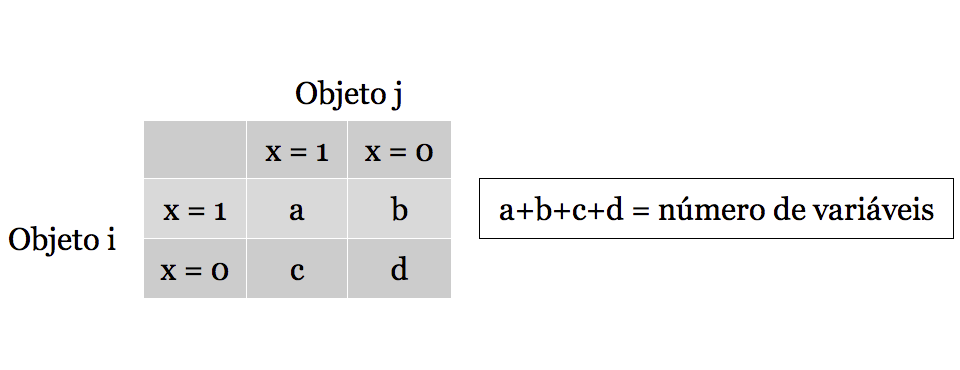
\includegraphics[width=0.8\linewidth]{./figures/matriz_confusao}
\caption{Matriz confusão de dois objetos com atributos binários}
\label{fig:matriz_confusão}
\end{figure}


Os atributos binários ainda podem ser divididos em dois tipos de atributos diferentes, os simétricos e os assimétricos, sendo em seguido apresentado as funções distância para ambos oa casos~\citet{Liu2011}.

\begin{description}
\item[Atributos simétricos: ] Um atributo é simétrico quando ambos os estados (0 ou 1) têm a mesma importância e o mesmo peso, tal como ocorre no exemplo dado anterior com o atributo género (masculino e feminino). Para este caso, a função distância mais utilizada é designada por \textit{simple matching distance}, que corresponde à proporção de incompatibilidade ou desacordo(equação~\ref{eq:symetric}).  

\begin{equation}
 dist(x_{i}, x_{j}) =  \frac{b + c}{a + b + c + d}
 \label{eq:symetric}   
\end{equation}

\item[Atributos assimétricos: ] Um atributo é assimétrico se um dos estados apresenta maior importância ou valor do que o outro. Normalmente o estado mais valioso é o que ocorre com menor frequência. No nosso caso iremos considerar o estado 1 como o mais valioso. Assim, a função distância mais frequentemente utilizada para atributos assimétricos é a \textit{Jaccard distance}:

\begin{equation}
 dist(x_{i}, x_{j}) =  \frac{b + c}{a + b + c}
\label{eq:asymetric}   
\end{equation}

\end{description}

No caso de atributos nominais com mais de dois estados ou valores, a função distância mais utilizada, é baseada na \textit{simple matching distance}. Dado dois objetos \textit{i} e \textit{j}, \textit{r} corresponde ao número total de atributos e o \textit{q} ao número de valores que são mutuamente correspondidos entre os objetos \textit{i} e \textit{j}:

\begin{equation}
 dist(x_{i}, x_{j}) =  \frac{r + q}{r}
\end{equation}

\subsubsection{Dimensão Temporal}

O tempo é representado apenas por uma dimensão, sendo que para calcular a distância, por exemplo, entre dois tweets $ t_{i} $ e $ t_{j} $, apenas é necessário calcular a diferença dos tempos entre os mesmos. Supondo que os valores dos tempos são respetivamente $ \Delta_{i} $ e $ \Delta_{j} $, o intervalo de tempo pode ser definido pela seguinte equação:

\begin{equation}
dist^{T}( t_{i}, t_{j}) = |\Delta_{i} - \Delta_{j}|  
\end{equation}

Sendo que, para a dimensão temporal, também é possível utilizar a função distância euclidiana (equação~\ref{eq: euclid}).

\subsubsection{Dimensão Espacial}

Ao contrário da dimensão temporal, a dimensão espacial apresenta mais do que uma dimensão, latitude e longitude. Estas apresentam-se sobre a forma numérica, sendo possível o cálculo da distância entre dois objetos através de funções de distância para atributos numéricos como referido anteriormente (\ref{subsubsec: attrnum}). Assim, para o cálculo entre pontos distribuídos num espaço poderá-se-á recorrer à função Minkowski (equação~\ref{eq:mink}), à função Euclidiana (equação\ref{eq: euclid}, à função Manhattan (equação~\ref{eq: manhattan}) ou mesmo à função de Chebychev (equação~\ref{eq:cheby}), sendo que no caso mais específico de uma distribuição espacial geográfica, em que os pontos possuem latitude e longitude, é considerada mais apropriada a utilização da função distância Haversine (equação~\ref{eq:hav}) pois esta toma em consideração a forma esférica da Terra.
Obtendo um par de objetos $ x_{i} $ e $ x_{j} $ distanciados geograficamente, é considerado as latitudes $ \phi_{x_{i}} $ e $ \phi_{x_{j}} $ e longitudes $ \lambda_{x_{i}} $ e $ \lambda_{x_{j}} $ para determinar a distância através da seguinte equação,

\begin{equation}
dist^{Sp}( x_{i}, x_{j}) = 2R\sin^{-1}\left( \left[ \sin^{2}(\frac{\phi_{x_{i}}-\phi_{x_{j}}}{2})+\cos\phi_{x_{i}}\cos\phi_{x_{j}}\sin^{2}(\frac{\lambda_{x_{i}}-\lambda_{x_{j}}}{2})\right] ^{0.5}\right) 
\label{eq:hav} 
\end{equation}

onde $ R $ representa o raio da Terra e que determina as unidades do resultado retornado pela função, sendo comum a utilização das unidades no sistema internacional (SI), o metro, podendo também ser representado em quilómetros devido ao fator de escala. 

% clocar uma bibliografia para a formula


% % escrever depois
%\subsubsection{Avaliação de Clusters}


% % % NOVA SECÇÃO % % %

\section{TweeProfiles} \label{sec:tweep}

Esta dissertação pretende dar continuidade e um trabalho designado por TweeProfiles. O TweetProfiles é uma ferramenta de análise e visualização espaço-temporal de dados recolhidos no Twitter. Esta secção faz um breve introdução e descrição sobre esta ferramenta.

\subsection{Objetivos}



\subsection{Descrição}

\subsection{Resultados ilustrativos}

\subsection{Prós e contras}

% % % NOVA SECÇÃO % % %

\section{Representação de informação visual} \label{sec:represent}

Na secção~\ref{sec:cluster} foi apresentado o conceito e características da tarefa de \textit{clustering} de uma forma geral. Nesta secção será exposto formas de representar imagens como dados. É importante salientar que a tarefa de \textit{clustering} em imagem é muitas vezes associada à técnica de segmentação de imagem~\citet{Forsyth2011}, não sendo este o objetivo deste projeto de dissertação, onde se pretende que para tarefa de \textit{clustering} cada objeto seja considerado a imagem no seu conjunto. 

\subsection{Representação matricial} \label{subsec:matrix}

Uma imagem pode ser vista como um objeto (ou instância), sendo computacionalmente representada como uma matriz (um vetor bi-dimensional) de pixels. A matriz de pixels descreve assim a imagem como N x M \textit{m}-bit pixels, onde N corresponde ao número de pontos ao longo do eixo horizontal, M o número de pontos ao longo do eixo vertical e \textit{m} o número de bits por pixel que controla os níveis de brilho. Com \textit{m} bits temos uma gama de valores para o brilho de $ 2^m $, que varia entre 0 e $ 2^m - 1 $. Assim se o valor de \textit{m} for 8, os valores de brilho de cada pixel de uma imagem podem variar entre 0 e 255, que normalmente correspondem ao preto e branco respetivamente, sendo que os valores intermédios correspondem ao tons de cinza~\citet{Nixon2002}.

No caso de imagens a cores, o principio é idêntico, no entanto ao invés de se usar apenas um plano, as imagens a cores são representadas por 3 componentes de intensidade, designado por modelo \textit{RGB}, a que corresponde respetivamente às cores vermelho (Red), verde (Green) e azul (Blue). Para além deste esquema de cores, também existe outros como o CMYK composto pelas componentes de cor, azul turquesa, magenta, amarelo e preto. Usando qualquer esquema de cores, existem 2 métodos principais para representar a cor do pixel. No primeiro método é utilizado um valor inteiro para cada pixel, sendo esse valor como um índice para uma tabela, também conhecida como palete da imagem, com a correspondência à intensidade de cada componente de cor. Este método tem como vantagem o facto de ser eficiente na utilização da memória, pois apenas é guardado um plano da imagem (os índices) e a palete (tabela). Por outro lado, tem como desvantagem o facto de normalmente ser usado um conjunto reduzido de cores o que provoca uma redução da qualidade da imagem. Já o segundo método consiste na utilização de vários planos da imagem para armazenar a componente de cor de cada pixel. Este representa a imagem com mais precisão pois considera muito mais cores.  Formato mais usual é 8 bits para cada uma das 3 componentes, no caso do RGB. Assim, são utilizados 24 bit para representar a cor de cada pixels, o que permite que uma imagem possa conter mais de 16 milhões de cores simultaneamente. Como era de esperar, isto envolve um custo grande na utilização de memória, mas a constante redução do custo das memórias faz com que este seja uma boa alternativa à apresentada anteriormente~\citet{Nixon2002}.

\subsection{Histogramas} \label{subsec:hist}

Outras das formas de representar a informação de uma imagem é através de um histograma. Um histograma de uma imagem apresenta a frequência de ocorrência de níveis individuais de brilho, representado através um gráfico que mostra o número de pixels da imagens com um determinado nível de brilho. No caso de pixels representados por 8-bit, o brilho vai variar de 0 (preto) até 255 (branco)~\citet{Nixon2002}. Também pode ser apresentado informação de cor sobre uma imagem através de um histograma, sendo para isso necessário apresentar 3 histogramas diferenciados, um para cada componente de cor, no caso do esquema RGB.
A figura~\ref{fig:lenahist} apresenta um exemplo de um histograma de uma imagem com tons cinza, onde são representados o número de pixeis para cada nível diferente de cinzento.

\begin{figure}[h]
\centering
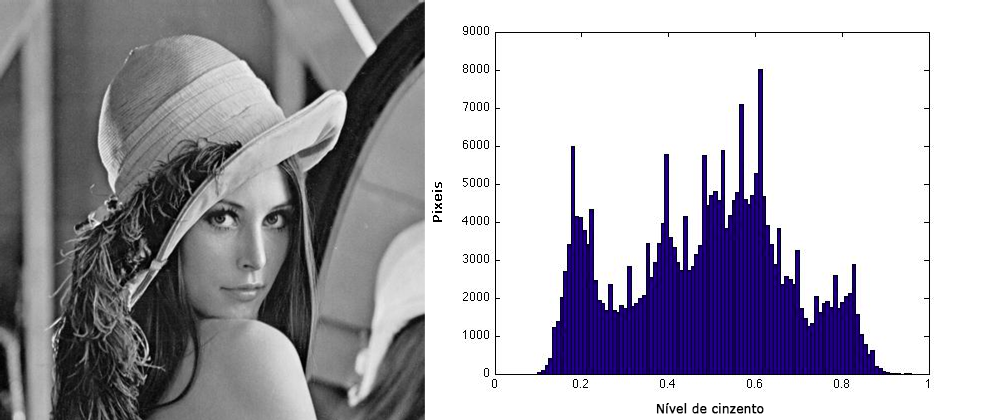
\includegraphics[width=0.8\linewidth]{./figures/histlena}
\caption{Imagem em tons cinza e respetivo histograma }
\label{fig:lenahist}
\end{figure}

\subsection{Descritores de cor}

A cor apresenta-se como um importante atributo da imagem para o olho humano e processamento por computador. Nesta subsecção são apresentados vários descritores de cor, utilizados para extração de informação e reconhecimento de similaridade em imagens. Por exemplo, o histograma de cores, referido na subsecção anterior~\ref{subsec:hist}, é um dos descritores de cor mais utilizados para caracterizar a distribuição da cor de uma imagem, mas apresenta uma baixa eficiência. Assim, em seguida é apresentado descritores de cor considerados pelo MPEG-7~\cite{Manjunath2001, Christopoulos2000, Cieplinski2001, Ite-vil}, que apresentam eficiência superior aos histogramas de cor.


\subsubsection{Espaços de cor} \label{subsubsec:space}

Nesta subsecção é apresentado os vários descritores de espaços de cor especificado no MPEG-7~\cite{Ite-vil}. Existe uma vasta seleção de espaços de cores, tais como, RGB, YCbCr, HSV, HMMS, Monocromático e Matriz linear de transformação com referência a RGB. Estes são usados por outro descritor de cor, mais especificamente, o descritor de dominância de cor que será falado posteriormente. É utilizado também, um sinalizador para indicar a referência a uma cor primária e de mapeamento de um valor de referência do branco padrão. 

Em espaços de cor, as componentes de cor são definidas como entidades de valor continuo, sendo que podem ser representadas por valores discretos através de uma quantização uniforme, em que é especificado um número de níveis de quantização para cada componente de cor no espaço de cor. A única exceção é o espaço de cor HMMD.

O espaço de cor RGB é um dos modelos referidos mais utilizados, que apresenta três componentes distintas, vermelho, verde e azul, tal como foi referido no subsecção~\ref{subsec:matrix}. Neste modelo é utilizado a combinação das 3 cores primárias para representar as diferentes cores. O modelo YCbCr provém do padrão MPEG-1/2/4~\cite{Ite-vil} e é definido pela transformação linear do espaço de cor RGB como demonstrado na equação~\ref{eq:ycbcr}:

\begin{eqnarray}
&& Y = 0.299\times R + 0.587\times G + 0.114\times B\nonumber\\
&& Cb = -0.169\times R - 0.331\times G + 0.500\times B \nonumber\\
&& Cr = 0.500\times R - 0.419\times G - 0.081\times B \label{eq:ycbcr}
\end{eqnarray} 

Para o espaço de cor Monocromático, é usado apenas a componente Y do modelo YCbCr. 

O espaço de cor HSV apresenta uma especificação mais complexa, tendo sido desenvolvido para fornecer uma representação mais intuitiva e para se aproximar mais do sistema visual humano. A transformação do modelo RGB para o HSV não é linear, mas é reversível~\cite{Manjunath2001}. Uma das componentes é a matiz (H - \textit{Hue}), que representa a componente de cor espectral dominante na sua forma mais pura, como o verde, amarelo, azul e vermelho. Ao ser adicionado branco à cor, esta sofre uma alteração, sendo que, adicionando mais branco, menos saturada se torna a cor. A saturação (S - \textit{Saturation}) é precisamente outra das componentes deste modelo. Por fim, o valor (V - \textit{Value}) corresponde ao brilho de cor.

O espaço de cor HMMD (\textit{Hue-Max-Min-Diff})~\cite{Manjunath2001, Ite-vil} é mais recente, que é caracterizado pela componente matiz, tal como o modelo HSV, pelo \textit{max} e \textit{min}, que são respetivamente o máximo e mínimo entre os valores R, G e B. Para descrever este modelo, também é utilizado a componente \textit{Diff}, que corresponde à diferença entre o \textit{max} e \textit{min}. Para representar este espaço de cor, apenas é necessário três dos quatro componentes referidos anteriormente, como por exemplo, {\textit{Hue, Max, Min}} ou {\textit{Hue, Diff, Sum}}, onde \textit{Sum} pode ser definida pela equação~\ref{eq:sum}.

\begin{equation}
Sum = \frac{Max + Min}{2}
\label{eq:sum}
\end{equation}

\subsubsection{Cor dominante}

O descritor de cor dominante fornece uma compacta representação das cores de uma imagem ou da região da imagem. Este apresenta a distribuição das cores mais representativas na imagem. Ao contrário do descritor de cor por histograma, na especificação do descritor de cor dominante, as cores mais representativas são calculadas a partir de cada imagem, em vez de ser fixado no espaço de cor, permitindo assim, uma representação das cores mais exatas e compacta, presentes numa região de interesse.

O descritor de cor dominante pode ser definido como,
\[ F = {{c_{i}, p_{i}, v_{i}},s}, (i=1,2,...,N) \]
onde N é o número de cores dominantes. Cada valor $ c_{i} $ da cor dominante é um vetor de valores das componentes do espaço de cor correspondente (por exemplo, um vetor de 3 dimensões no espaço de cor RGB). O valor $ p_{i} $ é a fração de pixels na imagem ou região da imagem (normalizado para um valor entre 0 e 1) que corresponde à cor $ c_{i} $, sendo $  \sum_i p_{i} = 1 $. O opcional $ v_{i} $ descreve a variação dos valores de cor dos pixels em um \textit{cluster} em torno da cor representativa correspondente. Por fim, a coerência espacial $ s $ é um único número  representa a homogeneidade espacial global das cores predominantes na imagem~\cite{Ite-vil}.

\subsubsection{Cor escalável}

O descritor de cor escalável, pode ser interpretado como um esquema de codificação base que recorre à transformada de Haar, onde é aplicada aos valores do histograma de cor no espaço de cor HSV (referido na subsecção~\ref{subsubsec:space}). De uma forma mais especifica, o descritor de cor escalável, extrai, normaliza e mapeia de forma não linear os valores do histograma, numa representação inteira a 4-bit, dando assim mais relevância a valores mais pequenos. A transformada de Haar, é assim aplicada aos valores inteiros a 4-bit através das barras do histograma. 

A extração do descritor é realizada com computação um histograma de cor com 256 níveis no espaço de cor de HSV com a componente matiz (H) quantificada a 16 níveis, e a saturação (S) e o valor (V) quantificado cada um para 4 níveis~\cite{Christopoulos2000}. 

A aplicação típica do descritor, inclui como por exemplo, a busca de similaridade numa base de dados com conteúdo multimédia e pesquisa em enormes base de dados. 

\subsubsection{Grupo de \textit{Frames} / Grupo de Imagens}

O descritor de cor Grupo de Frames / Grupo de Imagens (GoF/GOP) é sobretudo utilizado para a representação conjunta de cores para várias imagens ou várias \textit{frames} de um segmento de vídeo, contíguas ou não contíguas. Este baseia-se em histogramas, que capturam de forma confiável o conteúdo da cor de várias imagens ou \textit{frames} de vídeo. Normalmente para um grupo de \textit{frames} ou imagens, é selecionado uma frame chave ou imagem chave, que representará as características relacionadas com o grupo. Os métodos são altamente dependentes da qualidade da seleção da amostra representativa, o que pode levar a resultados pouco fiáveis caso não seja bem executada~\cite{Ite-vil}.

A estrutura do descritor GoF / GoP é idêntica à do cor escalável, com a exceção do campo agregação, que especifica como os pixels da cor de diferentes imagens/\textit{frames} foram combinadas antes da extração do histograma de cor. Os valores possíveis são média, mediana e cruzamento. 

Uma das aplicações deste descritor, é a pesquisa em conjuntos grandes de imagens, para encontrar \textit{clusters} de imagens semelhantes através da cor, em que é utilizado a interseção de histogramas como medida de similaridade da cor. A interseção de histogramas é obtido calculando o valor mínimo de cada barra de cor do histograma ao longo das \textit{frames}/imagens e atribui esse valor às barras de cor do histograma resultante. A interseção encontra as cores mínimas comuns nas \textit{frames}/imagens, e portanto, pode ser utilizado em aplicações que requerem a deteção de um elevado grau de correlação da cor~\cite{Christopoulos2000}. 

\subsubsection{Estrutura de cor}

Este descritor é uma generalização do histograma de cores, que apresenta algumas características espaciais da distribuição de cores em uma imagem. Este tem a particularidade de, para além de apresentar o conteúdo da cor de forma semelhante a um histograma de cor, também apresentar informações sobre a estrutura de uma imagem, sendo esta a característica diferenciadora deste descritor de cor. Em vez de considerar cada pixel separadamente, o descritor recorre a uma estrutura de 8x8 pexels que desliza sobre a imagem. Ao contrário do histograma de cor, este descritor consegue distinguir duas imagens em que uma determinada cor está presente em quantidades iguais, mas que apresenta uma estrutura num dos grupos de pixels 8x8 com uma cor diferente nas duas imagens. Os valores de cores são representadas no espaço de cor HMMD com cone duplo, sendo o espaço quantificado de maneira não uniforme em 32, 64, 128 ou 256 níveis. 
Cada valor de amplitude de um nível é representado por um código de 8 bits. Este descritor apresenta um bom desempenho na tarefa de recuperação de imagens baseado na similaridade~\cite{Modi2008}.

\subsubsection{Disposição de cor}

O descritor de disposição de cor, caracteriza a distribuição espacial de cor de uma imagem. Este usa um vetor de cores representativas de uma imagem, expressas no espaço de cor YCbCr. O tamanho do vetor é fixado em 8x8 elementos para garantir invariância da escala do descritor. As cores representativas da imagem podem ser selecionadas de diversas maneiras, mas a mais simples é através do cálculo da média de cor do bloco de imagem correspondente. O descritor disposição de cor, pode ser usado para em pesquisa rápida de bases de dados de imagens~\cite{Cieplinski2001}.

%talvez necessite de melhorar

\subsection{Descritores de textura}

A textura das imagens é uma característica visual importante, que tem muitas aplicações na recuperação, navegação e indexação de imagens. Existem três descritores de textura, referenciados na norma MPEG-7~\cite{Wu2001}. Em seguida é apresentada uma pequena descrição dos mesmos.

\subsubsection{Descritor de textura homogénea}

O descritor de textura homogénea (HTD - \textit{Homogeneous Texture Descriptor}) descreve a distribuição estatística da textura de uma imagem. Existem neste descritor 62 interfaces de recurso, sendo 2 no domínio espacial e 60 no domínio das frequências. No domínio espacial, é extraído a média e o desvio padrão de uma imagem. No domínio das frequências, o espaço é dividido em 30 canais, sendo calculado o valor energético e o valor do desvio de energia da resposta do filtro Gabor em cada canal~\cite{Wu2001, Shao2009}. Este desenho baseia-se no facto de a resposta do córtex visual possuir banda limitada e do facto de o cérebro decompor o espectro em bandas na frequência espacial~\cite{Wu2001}.
O descritor de textura homogénea é essencialmente utilizado em aplicações de recuperação de imagens por similaridade. 

\subsubsection{Descritor de histograma de borda}

O descritor de histograma de borda (EHD - \textit{Edge Histogram Descriptor}) apresenta-se sobre a forma de um histograma de 80 níveis, que representa a distribuição de borda local de uma imagem. Este descreve as bordas em cada sub-imagem. Estas sub-imagens são obtidas através da divisão da imagem numa grelha 4x4 como pode ser visto na figura~\ref{fig:ehd}. Existem 5 tipos de classificação diferentes das bordas de cada sub-imagem, sendo elas: vertical, horizontal, 45-graus, 135-graus e não direcional~\cite{Wu2001}. 

Este descritor é utilizado na recuperação de imagens, como por exemplo, imagens naturais ou de esboço, devido à sua textura homogénea. É também suportado por este descritor, a pesquisa baseada em blocos de imagem.  

\begin{figure}
\centering
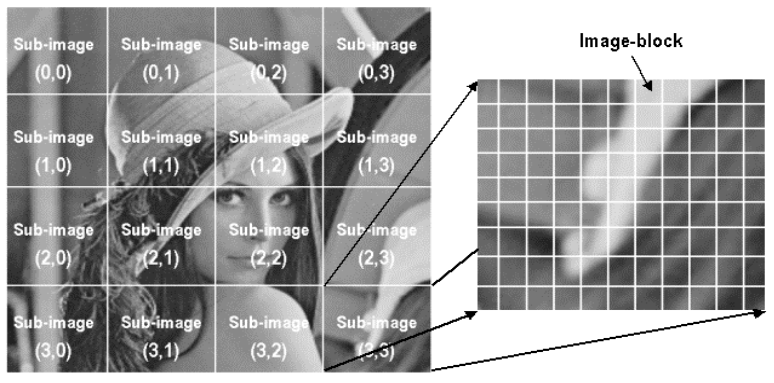
\includegraphics[width=0.7\linewidth]{./figures/ehd}
\caption{Sub-imagem e bloco de imagem. \textit{Retirada de}~\cite{Wu2001}}
\label{fig:ehd}
\end{figure}

\subsubsection{Descritor de navegação percetual}

O descritor de navegação percetual (HTD - \textit{Perceptual Browsing Descriptor}) foi projetado para navegação em base de dados, mas principalmente para quando essa navegação necessita de recursos com sentido percetual~\cite{Wu2001}. Este descritor é bastante compacto, que requer apenas 12 bits (máximo) para caracterizar regularidade (2 bits), direcionamento (3 bits x 2) e grosseirismo (2 bits x 2) da textura de uma imagem. A regularidade de uma textura pode apresentar valores numa escala entre 0 e 3, em que 0 indica uma textura irregular ou aleatória e 3 indica um padrão com direção e grosseirismo bem definidos. O direcionamento de uma textura é quantizada em 6 valores, variando de 0 a 150 em degraus de 30. Por fim, o grosseirismo de uma textura está relacionado com a escala e resolução de uma imagem. É quantizado em 4 níveis de 0 a 3, sendo 0 para um grão fino e 3 para uma textura grosseira. Estes valores têm uma relação com a divisão do espaço de frequência usado no cálculo do descritor de textura homogénea (HTD)~\cite{Manjunath2001}

\subsection{Descritores de forma}

O descritores de forma são dos descritores mais poderosos no reconhecimento de objetos. Isto deve-se ao facto de os seres humanos serem exímios no reconhecimento de objetos característicos exclusivamente através da suas formas, provando que a forma muitas vezes possui informação semântica~\cite{Bober2001}.  

\subsubsection{Descritor de forma baseado em região}
O descritor de forma baseado em região (RSD - \textit{Region-based Shape Descriptor})~\cite{Bober2001} apresenta a distribuição de um pixel dentro de uma região de um objeto em 2 dimensões. Este permite a descrição de objetos simples, com ou sem buracos (figura~\ref{fig:shape1}), mas também permite a descrição de objetos mais complexos, que contém múltiplas regiões sem ligação.

\begin{figure}[h]
\centering
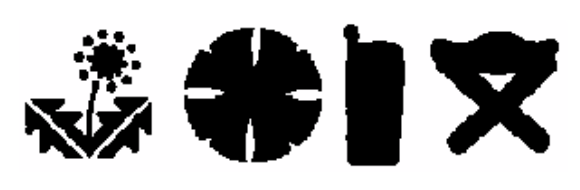
\includegraphics[width=0.7\linewidth]{./figures/shape1}
\caption{Exemplo de formas de objetos que podem ser descritas eficazmente pelo descritor baseado em região. \textit{Retirada de}~\cite{Bober2001} .}
\label{fig:shape1}
\end{figure}

As principais características deste descritor são~\cite{Bober2001}:

\begin{itemize}
\item Fornece uma forma compacta e eficiente de descrever várias regiões disjuntas;
\item Quando, no processo de segmentação de um objeto, ocorrem sub-regiões sem ligação, o objeto ainda pode ser recuperado, desde que a informação de quais as regiões que foram divididas seja mantida e usada na extração do descritor;
\item Apresenta uma boa robustez à segmentação de ruído.
\end{itemize}

\subsubsection{Descritor de forma baseado no contorno}

O descritor de forma baseado no contorno (CSD - \textit{Contour-based Shape Descriptor})~\cite{Bober2001} fundamenta-se na representação da curvatura espaço-escala (CSS - \textit{Curvature Scale-Space}) do contorno. O contorno é uma propriedade importante na identificação de objetos semanticamente semelhantes. É também bastante eficiente em aplicações onde a forma de objetos são muito variáveis, ou quando por exemplo, existem deformações de perspetiva. Esta apresenta um boa eficiência mesmo perante a existência de ruído nos contornos. 

As principais características deste descritor são~\cite{Bober2001}: 

\begin{itemize}
\item Consegue distinguir objetos que apresentem formas semelhantes mas que a forma do contorno apresenta propriedades bem diferenciadoras;
\item Tem a capacidade de encontrar formas que são semanticamente similar para os seres humanos, mesmo quando existe uma significativa variabilidade intra-classe;
\item É eficiente mesmo em casos de deformações não rígidas;
\item É eficiente mesmo em casos de distorções do contorno devido a variações de perspetiva, sendo uma situação muito comum em imagens e vídeo.
\end{itemize}
%(3D SD - 3-D Shape Descriptor)

\subsection{Descritores locais}

Um descritor local permite a localização das estruturas locais de uma imagem de forma repetitiva. Estas são codificadas de modo a que sejam invariantes a transformações das imagens, tais como a translação, rotação, mudanças de escala ou deformações. Assim, estes descritores podem ser utilizados para representar uma imagem e podem ser utilizados para diversos fins, tais como, reconhecimento de objetos, reconhecimento de cenas, perseguição de movimento, correspondência entre imagens ou mesmo obtenção de estruturas 3D de múltiplas imagens. 
Para a extração das características deste descritor é necessário utilizar um processo com as seguintes etapas~\cite{Gauman2010}:

\begin{itemize}
\item Encontrar um conjunto de pontos chave;
\item Definir uma região em torno de cada ponto-chave numa escala invariante;
\item Extrair e caracterizar o conteúdo da região;
\item Calcular o descritor da região normalizada;
\item Combinar os descritores locais.
\end{itemize}

Em seguida são apresentados duas das técnicas mais representativos dos descritores locais, o SIFT e o SURF.

\subsubsection{SIFT} \label{subsubsec:sift}

O descritor SIFT (\textit{Scale-invariant feature transform})~\cite{Lowe1999, Lowe2004} é um descritor local que transforma uma imagem numa grande coleção de vetores de características locais invariantes a translação, rotação, mudanças de escala, e parcialmente invariante a mudanças de iluminação. Pode assim ser utilizado para detetar correspondência entre imagens com diferentes visões de objetos ou cenas.
Este descritor apresenta como característica interessante o facto de compartilhar uma série de propriedades em comum com as respostas dos neurónios do lobo temporal na visão dos primatas. Os pontos-chave SIFT derivados de uma imagem são usados na indexação numa abordagem de vizinho mais próximo, para encontrar objetos candidatos. O modelo recorre a uma votação pela transformada Hough e a uma estimativa final pelo método dos mínimos quadrados. Quando 3 pontos chave estiverem em acordo, pode se afirmar que existe uma forte possibilidade da presença de um objeto.
Como foi indicado anteriormente, são necessários levar a cargo uma lista de etapas bem definidas para obtenção de descritores locais, sendo que as etapas para o descritor SIFT as seguintes:

\begin{enumerate}
\item \textbf{Deteção de extremos}:  A deteção de extremos (máximos e mínimos) é conseguida através da procura realizada em várias escalas e localizações, de modo a serem extraídos pontos de interesse invariáveis à escala e rotação, através da diferença de filtros gaussianos. Estes pontos de interesse ou pontos chave correspondem a estes extremos para várias escalas. 
Um filtro gaussiano passa baixo é dado pela convolução entre uma imagem \textit{I} e a função \textit{G}:

\begin{equation}
L\left ( x, y, \sigma  \right ) = G\left ( x, y, \sigma  \right ) * I\left ( x, y \right )
\end{equation}

onde ,
\begin{equation}
G\left ( x, y, \sigma  \right ) = \frac{1}{2\pi \sigma^2} e^\frac{-\left ( x^2 + y^2 \right )}{2\sigma^2} 
\end{equation}

em que o o filtro varia à escala através do parâmetro teta

A função \textit{DoG} (\textit{"Diference of Gaussian"}) é dada pela diferença entre as imagens filtradas em escalas próximas separadas por uma constante \textit{k} e pode ser definida como:

\begin{equation}
DoG\left ( x, y, \sigma  \right ) = G\left ( x, y, k\sigma  \right ) * G\left ( x, y, \sigma \right )
\end{equation}

Assim, a convolução de uma imagem \textit{I} com o filtro \textit{DoG} é dado por:

\begin{equation}
D\left ( x, y, \sigma  \right ) = \left (  G\left ( x, y, k\sigma  \right ) - G\left ( x, y, \sigma \right ) \right )* I\left ( x, y \right ) = L\left ( x, y, k\sigma  \right ) - L\left ( x, y, \sigma  \right )
\end{equation}

que corresponde à diferença entre as imagens filtradas pelo filtro gaussiano em escalas teta e $ k\sigma $. Este filtro provoca uma perda de nitidez nas imagens (efeito desfoque) e tornasse assim capaz de detetar variações de intensidade nas imagens, como por exemplo, nos contornos. A figura~\ref{fig:siftdog} mostra como é realizado o processo de obtenção das Diferenças Gaussianas e consequente formação das oitavas. 

\begin{figure}[h]
\centering
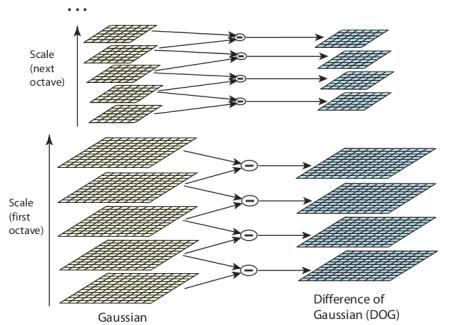
\includegraphics[width=0.7\linewidth]{./figures/sift_dog.jpg}
\caption{ Construção das Diferenças Gaussianas e formação de oitavas \textit{Retirada de}~\cite{Lowe2004} .}
\label{fig:siftdog}
\end{figure}

Segundo Lowe~\cite{Lowe2004}  é necessário atingir a escala $ 2\sigma $ para ser possível a construção de um descritor local invariável à escala, logo

$ k = 2^{\left(1/s \right)} $

onde s é o número de intervalos entre imagens obtidas por \textit{DoG} e $ D(x, y, \sigma) $ corresponde à primeira imagem e $ D(x, y, 2\sigma) $ à última de todo conjunto de imagens geradas. Também deverão ser assim obtidas $s + 3$ imagens na pilha de imagens filtradas para cada oitava. Cada oitava contém as imagens de Diferença Gaussiana, sendo as que ficam entre as escalas superiores e inferiores designadas de intervalo. 

Por fim é realizado o processo de deteção de extremos, onde um pixel é comprado com os seus oito vizinhos na imagem atual e com os nove pixeis vizinhos das imagens de escalas adjacentes, numa região de 3x3. A figura~\ref{fig:siftdog2} ilustra este processo.  

\begin{figure}[h]
\centering
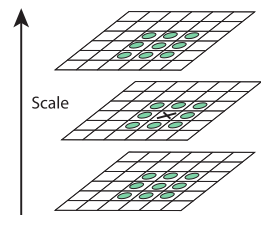
\includegraphics[width=0.4\linewidth]{./figures/sift_dog2.png}
\caption{Ilustração do processo de deteção de máximos e mínimos das imagens de Diferença Gaussiana. O pixel candidato está marcado com X e os vizinhos com um circulo. \textit{Retirada de}~\cite{Lowe2004}}
\label{fig:siftdog2}
\end{figure}

O próximo processo passa pela localização dos ponto chave.

\item \textbf{Localização de pontos chave}: quando detetado um extremo, esse ponto é considerado um candidato a ponto chave ou ponto de interesse. Este ponto foi encontrado através da comparação de um pixel com os seus vizinhos como referido anteriormente. sendo necessário realizar um cálculo de ajuste detalhado da localização e escala gaussiana de cada um destes pontos. É utilizada então a série de Taylor para obter uma localização mais exata dos extremos, sendo rejeitado caso a intensidade de um extremo seja inferior a um limiar previamente definido. 

Como DoG tem uma boa resposta a arestas e como estás fazem com que os pontos sejam instáveis com ruído, estes necessitam de ser removidos. É assim através da utilização uma matriz Hessiana 2x2 é possível com calcular as curvaturas principais. Caso o rácio seja superior a um limiar previamente definido, é considerado uma aresta e assim o ponto chave é descartado.

Após a remoção de todos os pontos considerados não sendo de interesse, fica-se com todos os pontos chave, sendo necessário a atribuição das suas orientações. 

\item \textbf{Atribuição da orientação dos descritores}: este processo tem como principal finalidade possibilitar a representação de um descritor em relação a sua orientação, permitindo assim que este seja invariante a rotações. Para realizar esta tarefa é utilizada a escala Gaussiana $ \sigma $ para a escolha da imagem filtrada \textit{L} com a escala mais próxima e com a oitava referente ao ponto avaliado, tornando assim invariante também à escala.

Assim são calculados os gradientes para cada imagem $ L(x, y, \sigma) $ de intervalo, referentes às escalas e oitavas utilizadas.

A magnitude e orientação são calculados da seguinte forma:

\begin{equation}
m(x,y) = \sqrt{\left ( \left ( L(x+1, y) - L(x-1, y) \right )^2 + \left ( L(x, y+1) - L(x, y-1) \right )^2  \right )}
\end{equation}

\begin{equation}
\theta (x, y) = tan^{-1}\left ( \frac{\left ( L(x, y+1) - L(x, y-1) \right )}{\left ( L(x+1, y) - L(x-1, y) \right )} \right )
\end{equation}

Assim, é criado um histograma das orientações para pixeis numa região em redor do pontos chave, em que de todas as orientações obtidas para um ponto, apenas o maior pico e aquelas acima de 80\% do valor desse pico é que são utilizadas para definir a orientação de cada ponto chave.

Por fim, é possível a construção dos descritores para os pontos chave definidos como o ponto a seguir apresenta.

\item \textbf{Construção do descritor local}: este é o ultimo passo em que é criado o descritor local para cada ponto de interesse. Para esse processo, é considerado um bloco 16x16 em redor do ponto chave e posteriormente dividido em 16 sub-blocos de 4x4. Por cada sub-bloco é criado um histograma com 8 picos relativos à orientação. Isto faz que no fim seja extraído um vetor de 128 posições para cada ponto chave. Para além deste retorno, são também tomadas várias medidas de modo a que exista robustez suficiente para que esse ponto de interesse seja invariante a mudanças de iluminação e rotação. 

\begin{figure}
% %falta imagem
\end{figure}
 
\end{enumerate}

O algoritmo SIFT é regularmente utilizado em reconhecimento de objetos ou cenas, tendo sido utilizado em deteção de objetos em \textit{frames} de vídeo~\cite{Sivic2003, Sivic2006} com utilização de técnicas mais avançadas de deteção de objetos e cenas utilizando vocabulários visuais como é apresentado na secção~\ref{subsec: vocab}.

%% SURF %% 
\subsubsection{SURF} \label{subsubsec:surf}

Outro algoritmo importante de extração de descritores locais é o SURF (\textit{Speeded Up Robust Features}). Este é baseado no SIFT apresentado na subsecção anterior~\ref{subsubsec:sift} e também é utilizado, por exemplo, em reconhecimento de objetos ou mesmo na reconstrução 3D. Segundo os autores~\cite{Bay2006} o SURF é mais rápido (cerca de dez vezes) e robusto do que o SIFT, sendo que, segundo a comparação realizada em~\cite{Juan2009} comprovou-se que o SIFT é mais lento e não muito bom a mudanças de iluminação, mas apresenta melhores resultados a variações de rotação, mudanças de escala e transformações na imagem.

Este usa a técnica da imagem integral, onde cada pixel de uma imagem recebe um valor igual à soma dos pixeis da sua esquerda e acima, incluindo o próprio. Este também utiliza um filtro Haar em formato de caixa numa sub-região 4x4 em redor de um ponto de interesse, como se pode ver na figura~\ref{fig:surf}, tornando o processo computacionalmente eficiente. Isto é realizado calculando a soma das respostas dos filtros e a soma do modulo das respostas dos filtros nas direções horizontal e vertical, gerando assim 4 valores por cada sub-região. Logo, o SURF retorna um vetor de 64 dimensões, metade do retornado pelo algoritmo SIFT.

\begin{figure}[h]
\centering
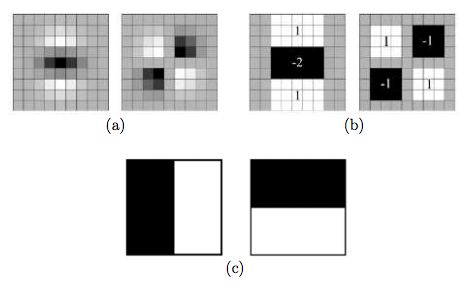
\includegraphics[width=0.7\linewidth]{./figures/surf}
\caption{ (a) Filtros Gaussianos de segunda ordem nas direções yy e xy; (b) aproximação por filtros de caixa; (c) filtros de Haar; As regiões a cinzento têm valor igual a zero. \textit{Retirada de}~\cite{Bay2006}.}
\label{fig:surf}
\end{figure}

Para além destes dois algoritmos ainda existe outros menos utilizados como o GLOH (\textit{Gradient Location and Orientation Histogram}) e o HOG (\textit{Histogram of Oriented Gradients}).

Na próxima secção e apresentado

\subsection{Descritores baseado em vocabulário visual}\label{subsec: vocab}

No reconhecimento de documentos de texto é utilizado o conceito de vocabulário textual, sendo muitas vezes designado por \textit{bag of words} que em português significa, saco de palavras, onde existe um conjunto de palavras armazenadas pré definidas. Um texto é assim caracterizado, através da análise das palavras que possui, sendo contabilizado a frequência de palavras que estejam simultaneamente no texto e no \textit{bag of words}, que assim atribuem um significado ao texto. É também utilizado uma lista de palavras que não acrescentam significado a expressões tais como, "o" ou "um", entre outras, que são removidas do texto durante a análise para não influenciarem os resultados. Um sistema de extração de informação de texto apresenta um número padrão de etapas~\cite{Baeza-Yates1999}. 

Recentemente esta técnica foi adotada em aplicações de extração de informação visual, como por exemplo é nos mostrado em~\cite{Sivic2003, Sivic2006}. Esta recorre a descritores locais invariantes a escala e rotação, para criar um vocabulário visual. A utilização de descritores locais como o SIFT, referido na secção anterior anterior~\ref{subsubsec:sift}, permite a extração de pontos de interesse nas imagens, invariantes a rotação e mudanças de escalas.

Quando efetuado este processo repetidamente com um grande conjunto de imagens, é possível criar \textit{clusters} de regiões de imagens muito semelhantes entre si, como se pode ver na figura~\ref{fig:visualword}. Todas estas regiões são candidatas a palavras visuais, sendo selecionada a que representa melhor esse \textit{cluster}, isto é, é selecionado o centroide desse conjunto de regiões semelhantes entre si, recorrendo ao algoritmo \textit{k-means} referido na secção~\ref{subsec:parti}. Esse centroide passa então a ser considerado uma palavra visual e é adicionado a um vocabulário com outras palavras visuais.

\begin{figure}[h]
\centering
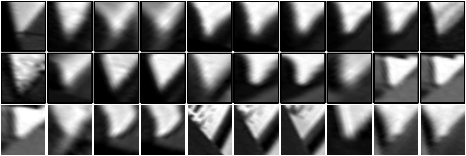
\includegraphics[width=0.4\linewidth]{./figures/visual_word_1}
\label{fig:visualword}
\end{figure}

%\begin{figure}[h]
%	\centering
%	\begin{subfigure}[b]{0.4\textwidth}
%		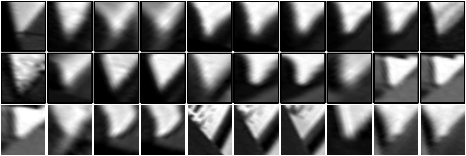
\includegraphics[width=\textwidth]{./figures/visual_word_1}
%		\caption{ }
%	\end{subfigure}
%	\quad
%	\begin{subfigure}[b]{0.4\textwidth}
%		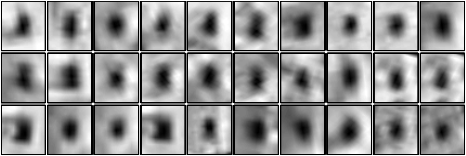
\includegraphics[width=\textwidth]{./figures/visual_word_2}
%		\caption{ }
%	\end{subfigure}
%	
%	\begin{subfigure}[b]{0.4\textwidth}
%		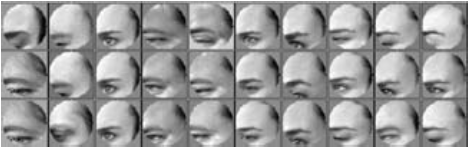
\includegraphics[width=\textwidth]{./figures/visual_word_3}
%		\caption{ }
%	\end{subfigure}
%	\quad
%	\begin{subfigure}[b]{0.4\textwidth}
%		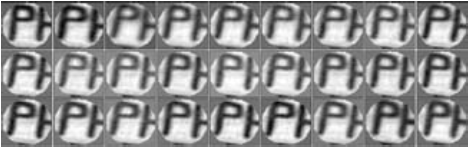
\includegraphics[width=\textwidth]{./figures/visual_word_4}
%		\caption{ }
%	\end{subfigure} 
%	\caption {Amostras de regiões com variância conjunta normalizadas de grupos que correspondem a uma única palavra visuais. \textit{Retirada de}~\cite{Sivic2006}}
%	\label{fig:visual_word}
%\end{figure}

Por fim é necessária a realização de uma indexação de cada palavra visual às imagens, sendo utilizado um vetor para cada imagem que indica, o número de vezes em que uma determinada palavra visual se repete numa imagem. Neste caso o vetor funciona como em \textit{text mining}, em que existe a contagem da frequência de palavras que ocorrem num determinado documento.

Outro processo possível para indexação do conteúdo visual ou texto, é atribuição de um peso ou ponderação para cada palavra visual numa determinada imagem. Aqui é utilizado a ponderação padrão conhecida como tf-idf ('\textit{term frequency-inverse document frequecy}')~\cite{Sivic2003}. 

Considerando um vetor com \textit{k} palavras visuais $Vd = (t_{1},...,t_{i},...,t_{k})$, em que a ponderação de cada palavra é dada pela equação~\ref{eq:peso}

\begin{equation}
t_{i} = \frac{n_{id}}{n_{d}}log\frac{N}{n_{i}}
\label{eq:peso}
\end{equation}

onde $n_{id}$ é o numero de ocorrências da palavra \textit{i} num documento \textit{d}, $n_{d}$ o número total de palavras no documento \textit{d}, $n_{i}$ é o numero de ocorrências da palavra \textit{i} em todos documentos e \textit{N} é o numero de documentos existentes. 

Concluí-se assim que este descritor permite a identificação de imagens semelhante ou reconhecimento de objetos, através da comparação dos vetores de cada imagem, com a informação relativa ao vocabulário posteriormente criado. Este demonstra ser bastante eficiente, e segundo Nistér e Stewénius~\cite{Nister2006} é possível escalar este processo para enormes quantidades de imagens sem perda de performance utilizando para isso um vocabulário em forma de árvore, isto é, com a hierarquização das palavras visuais de um vocabulário visual, recorrendo para isso ao \textit{clustering} hierárquico.

%Para a criação deste vocabulário visual, as regiões selecionadas podem ter em conta dois tipos diferentes de pontos de vista visual~\cite{Sivic2003, Sivic2006}. Um é designado por \textit{Shape Adapted} (SA), em que a forma adaptada sobre um ponto de interesse é elíptica. Este envolve um método iterativo para determinar o centro, escala e forma da elipse. O segundo, é designado por \textit{Maximally Stable} (MS), que tem como característica o facto de as regiões selecionadas serem as que a área é aproximadamente estacionária entanto o limiar de intensidade varia. Assim, as regiões SA tendem a centrar-se nos cantos e as regiões MS correspondem a formas de alto contraste em relação ao seu redor, como pode ser visualizado nos exemplos da figura~\ref{fig:visual_word}.
%
%Conclui-se assim que o objetivo é quantizar os descritores em \textit{clusters} que serão as "palavras" visuais. O quantização vetorial pode ser realizado com recurso ao algoritmo de \textit{clustering} \textit{k-means} referido na secção~\ref{subsec:parti}, ou também a histogramas~\cite{Sivic2003, Sivic2006}.

%Utilizado este tipo de descritor, é possível identificar imagens semelhantes, através da contagem de regiões de pontos-chave co-existentes entre as imagens. 

%\section{Trabalhos relacionados} \label{sec:work}
%
%A extração de informação em imagens é realizada já à vários anos, sendo muito utilizada na pesquisa de informação. Existem muitos trabalhos que, mesmo tendo objetivos diferentes, apresentam uma forte relação com o objetivo deste projeto de dissertação.
%Uma das áreas que se pode encontrar trabalhos relacionados é na deteção de objetos em vídeos~\cite{Sivic2003, Sivic2006}, onde se pretende identificar cenas de filmes semelhantes, tanto no mesmo filmes, como entre filmes diferentes, recorrendo a descritores baseados em vocabulário visual.
%Como é de esperar, também existe vários trabalhos relacionados, que apresentam métodos diferentes para encontrar imagens semelhantes, como na pesquisa web~\cite{Cai2004, Gao2005}.
%Na pesquisa bibliográfica realizada, foram encontrados dois trabalhos onde existe uma forte relação com o objetivo do projeto, e que apresentam técnicas que demonstraram bons resultados.
%O primeiro~\cite{Nister2006} utiliza os descritores baseados em vocabulário visual, tendo como diferenciação, a utilização de uma árvore hierárquica para reconhecimento de imagens semelhantes. O segundo
%~\cite{Lin2014}, apresenta conjuntos de imagens semelhantes através da utilização do algoritmo de \textit{clustering}, \textit{k-means}, sendo que recorre a uma modificação que torna o algoritmo mais rápido, reduzindo o tempo de processamento mesmo com uma grande base de dados. Para a realização deste este trabalho, foi utilizado histogramas de cor e histogramas preto e branco para descrever as imagens e ser possível assim identificar semelhanças entre elas.

